\documentclass[10pt,landscape]{article}
\usepackage[utf8]{inputenc}
\usepackage[ngerman]{babel}
\usepackage{tikz}
\usetikzlibrary{shapes,positioning,arrows,fit,calc,graphs,graphs.standard}
\usepackage[nosf]{kpfonts}
\usepackage[t1]{sourcesanspro}
%\usepackage[lf]{MyriadPro}
%\usepackage[lf,minionint]{MinionPro}
\usepackage{multicol}
\usepackage{wrapfig}
\usepackage[absolute,overlay]{textpos}
\usepackage[top=4mm,bottom=8mm,left=4mm,right=4mm]{geometry}
\usepackage[shortlabels]{enumitem}
\usepackage[framemethod=tikz]{mdframed}
\usepackage{microtype}
\usepackage{amsmath}
\usepackage{mathtools}
\usepackage{dirtytalk}
\usepackage{listings}
\usepackage{hyperref}
\usepackage{comment}
\usepackage{wrapfig}


\usepackage{graphicx}

\let\bar\overline
\newcommand{\Lim}[1]{\raisebox{0.5ex}{\scalebox{0.8}{$\displaystyle \lim_{#1}\;$}}}

\DeclarePairedDelimiter\abs{\lvert}{\rvert}%
%\setlist[enumerate,1]{leftmargin=5mm}
\setlist[itemize,1]{leftmargin=5mm}
\setlength{\multicolsep}{6.0pt plus 2.0pt minus 1.5pt}%{6.0pt plus 2.0pt minus 1.5pt}% 50% of original values
\setlist{nosep}


\definecolor{myblue}{cmyk}{1,.72,0,.38}
\definecolor{mygrey}{RGB}{54,71,76}
\definecolor{vestablue}{HTML}{2B3F48}
\definecolor{pastelred}{HTML}{fbb4ae}
\definecolor{pastelblue}{HTML}{b3cde3}
\definecolor{pastelgreen}{HTML}{ccebc5}
\definecolor{pastelpurple}{HTML}{decbe4}
\definecolor{pastelorange}{HTML}{fed9a6}
\definecolor{pastelyellow}{HTML}{ffffcc}
\definecolor{pastelbrown}{HTML}{e5d8bd}
\definecolor{pastelpink}{HTML}{fddaec}
\definecolor{pastelgrey}{HTML}{f2f2f2}
\definecolor{forestgreen}{HTML}{228B22}

\tikzset{filled/.style={fill=circle area, draw=circle edge, thick},
    outline/.style={draw=circle edge, thick}}

\pgfdeclarelayer{background}
\pgfsetlayers{background,main}

\everymath\expandafter{\the\everymath \color{myblue}}
\everydisplay\expandafter{\the\everydisplay \color{myblue}}

\renewcommand{\baselinestretch}{.8}
\pagestyle{empty}

\global\mdfdefinestyle{header}{%
linecolor=gray,linewidth=1pt,%
%leftmargin=1mm,rightmargin=2mm,skipbelow=2mm,skipabove=2mm,
}

\newcommand{\header}{
\begin{mdframed}[style=header]
\footnotesize
\sffamily
\Large{\textbf{D3}} \footnotesize Cheatsheet\\
by~Blair~Labatt~III,~page~\thepage~of~2
\end{mdframed}
}

\newcommand{\subsec}[2]{
\subsection*{
\begin{minipage}{32mm}
#1
\end{minipage}
[\texttt{#2}]}
}

\newenvironment{code}
    {
    \fboxsep0pt
    \colorbox{pastelgrey}
    }
    {
    }

\newcommand{\mycol}[1]{%%%
    \begin{minipage}{12mm}%%
        #1%%%
    \end{minipage}%%%
}%%%

\newcommand{\mycolX}[2]{%%%
    \begin{minipage}{{#1}}%%
        #2%%%
    \end{minipage}%%%
}%%%


\newcommand{\entry}[3]{%%%
    \begin{minipage}{{#1}}%%
        \code{#2}%%%
    \end{minipage}%%%
    \% #3
}%%%
 

\newenvironment{tinylist}[2]
    {\footnotesize\begin{multicols}{#1}
    \setlength{\topskip}{0pt}
    \begin{itemize}[label={},leftmargin=1mm]
    #2
    }
    { 
    \end{itemize}\end{multicols} 
    }

 
 
\lstset{%
  basicstyle=\small\ttfamily,
  breaklines=false,
  backgroundcolor = \color{pastelgreen},
  language=[LaTeX]{TeX}
}

\makeatletter
\renewcommand{\section}{\@startsection{section}{1}{0mm}%
                                {1.8ex}%
                                {.6ex}%x
                                {\color{myblue}\sffamily\Large\bfseries}}
\renewcommand{\subsection}{\@startsection{subsection}{1}{0mm}%
                                {1.2ex}%
                                {.2ex}%x
                                {\sffamily\bfseries}}


\makeatother
\setlength{\parindent}{0pt}

\begin{document}

    
    
\small
\begin{multicols*}{4}
\header
\textit{D3 is rigorously declarative, but not purely functional. Most of the work is done in stateful \say{function objects}, of which $\exists$ 4 main types:}\begin{itemize}
    \item Factory\textsubscript{F}: implement prescribed APIs
    \item Generator\textsubscript{G}: Generate concrete visualization code (SVG, Canvas) from passed data
    \item Layout\textsubscript{L}: Transform passed dataset to include additional visual layout information
    \item Component\textsubscript{C}: Manipulate the DOM
\end{itemize}\textit{Subscripts are used herein to categorize D3 functions according to the above taxonomy.}

\section{\href{https://github.com/d3/d3-selection}{Data Joining \& Selections}}

%%%%%%%%%%%%%%%%%%%%%%%%%%%%%%%%%%%%%%%%%%%%%%%%%%%
\subsec{\href{https://github.com/d3/d3-selection\#selecting-elements}{Selecting}}{\href{https://observablehq.com/@d3/selection-join}{d3}}
\textit{Create a \href{https://bost.ocks.org/mike/selection/}{selection} with one of the following top-level calls, generally passing a \href{http://www.w3.org/TR/selectors-api/}{W3C} selector string:}

{\footnotesize 
\begin{minipage}[t]{2.0cm}
    selection\\
    selector\\
    window
\end{minipage}
\begin{minipage}[t]{2.0cm}
    select\\
    selectorAll\\
    style
\end{minipage}
\begin{minipage}[t]{2.0cm}
    selectAll\\
    matcher\\
\end{minipage}
}



\textit{Create derivative selections (subsets, unions, \href{https://bost.ocks.org/mike/nest/}{nestings}) by invoking one of the following methods of an already-existing selection:}

{\footnotesize 
\begin{minipage}[t]{1.5cm}
    select
\end{minipage}
\begin{minipage}[t]{1.5cm}
    selectAll
\end{minipage}
\begin{minipage}[t]{1.5cm}
    filter
\end{minipage}
\begin{minipage}[t]{1.5cm}
    merge
\end{minipage}
}


%%%%%%%%%%%%%%%%%%%%%%%%%%%%%%%%%%%%%%%%%%%%%%%%%%%
\subsec{\href{https://github.com/d3/d3-selection\#modifying-elements}{Modifying}}{\href{https://observablehq.com/@d3/selection-join}{<selection>}}

\textit{Change properties of DOM elements in bulk:}

{\footnotesize 
\begin{minipage}[t]{2.0cm}
    attr\\
    text\\
    insert\\
    sort\\
    lower
\end{minipage}
\begin{minipage}[t]{2.0cm}
    classed\\
    html\\
    remove\\
    order\\
\end{minipage}
\begin{minipage}[t]{2.0cm}
    property\\
    append\\
    clone\\
    raise\\
\end{minipage}
}


%%%%%%%%%%%%%%%%%%%%%%%%%%%%%%%%%%%%%%%%%%%%%%%%%%%
\subsec{\href{https://github.com/d3/d3-selection\#joining-data}{Joining}}{\href{http://bost.ocks.org/mike/join/}{<selection>}}

\href{https://bost.ocks.org/mike/circles/}{\resizebox{4cm}{!}{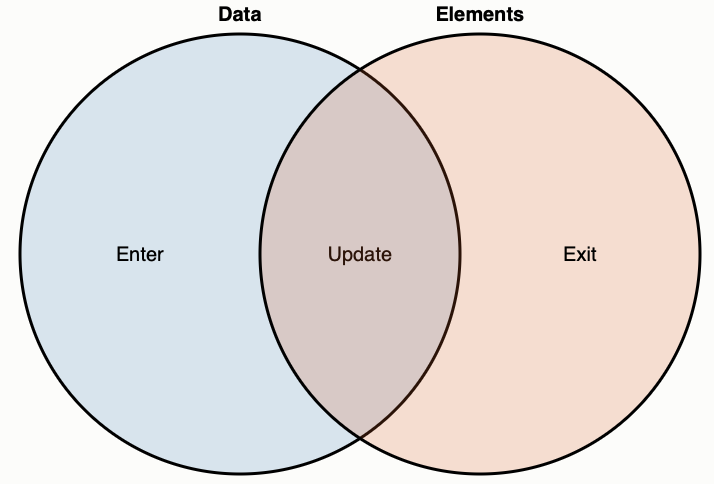
\includegraphics[]{img/gup.png}}}

\textit{The \href{https://bost.ocks.org/mike/join/}{\say{General Update Pattern}} involves a \say{data join}, followed by references to the resulting subset of elements \& data, and looks something like this:}

\code{svg.selectAll(\textquotedbl circle\textquotedbl)}\\
\code{\phantom{xx}.data(data)}\\
\code{\phantom{xx}.enter().append(\textquotedbl circle\textquotedbl)}\\
\code{\phantom{xxxx}.attr(\textquotedbl cx\textquotedbl , function(d) \{ return d.x; \})}\\
\code{\phantom{xxxx}.attr(\textquotedbl cy\textquotedbl , function(d) \{ return d.y; \})}\\
\code{\phantom{xxxx}.attr(\textquotedbl r\textquotedbl , 2.5);}\\

{\footnotesize 
\begin{minipage}[t]{1.2cm}
    data
\end{minipage}
\begin{minipage}[t]{1.2cm}
    join
\end{minipage}
\begin{minipage}[t]{1.2cm}
    enter
\end{minipage}
\begin{minipage}[t]{1.2cm}
    exit
\end{minipage}
\begin{minipage}[t]{1.2cm}
    datum
\end{minipage}
}

%%%%%%%%%%%%%%%%%%%%%%%%%%%%%%%%%%%%%%%%%%%%%%%%%%%
\subsec{\href{https://github.com/d3/d3-selection\#handling-events}{Events}}{d3}

\textit{Add/remove an event-handler with }\texttt{<selection>.on()}\textit{, or immediately dispatch an event with }\texttt{<selection>.dispatch()}\textit{. The following top-level functions return information about an active event:}

{\footnotesize 
\begin{minipage}[t]{2.0cm}
    event\\
    touch
\end{minipage}
\begin{minipage}[t]{2.0cm}
    customEvent\\
    touches
\end{minipage}
\begin{minipage}[t]{2.0cm}
    mouse\\
    clientPoint
\end{minipage}
}



%%%%%%%%%%%%%%%%%%%%%%%%%%%%%%%%%%%%%%%%%%%%%%%%%%%
\subsec{\href{https://github.com/d3/d3-selection\#control-flow}{Control}}{<selection>}

\textit{The following yield information about selections, except for }\texttt{each}\textit{ and }\texttt{call}\textit{, which afford arbitrary code execution for selections while maintaining the ability to chain subsequent methods.}


{\footnotesize 
\begin{minipage}[t]{2.0cm}
    each\\
    nodes
\end{minipage}
\begin{minipage}[t]{2.0cm}
    call\\
    node
\end{minipage}
\begin{minipage}[t]{2.0cm}
    empty\\
    size
\end{minipage}
}


%%%%%%%%%%%%%%%%%%%%%%%%%%%%%%%%%%%%%%%%%%%%%%%%%%%
\subsec{\href{https://github.com/d3/d3-selection\#local-variables}{Local Variables}}{\href{http://bl.ocks.org/mbostock/e1192fe405703d8321a5187350910e08}{<selection>}}

\textit{Afford the storage/retrieval of state that is independent of a selection\textquotesingle s data.}

{\footnotesize 
\begin{minipage}[t]{1.5cm}
    set
\end{minipage}
\begin{minipage}[t]{1.5cm}
    get
\end{minipage}
\begin{minipage}[t]{1.5cm}
    remove
\end{minipage}
\begin{minipage}[t]{1.5cm}
    toString
\end{minipage}
}


%%%%%%%%%%%%%%%%%%%%%%%%%%%%%%%%%%%%%%%%%%%%%%%%%%%
\subsec{Namespaces}{d3}

\textit{For use in construction XML namespaces.}

{\footnotesize 
\begin{minipage}[t]{2.0cm}
    namespace
\end{minipage}
\begin{minipage}[t]{2.0cm}
    namespaces
\end{minipage}
}

\section{Munging \& Formatting}

\textit{Data importation process can be complex. Here is a somewhat general pattern:}\\
\resizebox{6.5cm}{!}{%\begin{tikzpicture}[call/.style={
%rectangle,%minimum size=6mm,rounded corners=3mm, % The rest
%very thick,draw=black!50,
%top color=white,bottom color=black!20, font=\ttfamily}]

%    \graph[grow right sep, branch down=7mm]{
%        {data, nest/$d3.nest()$, file/$obs.FileAttachment()$} -> hier/$d3.hierarchy()$ -> tree/$d3.treemap()$ -> join/$d3.data()$;
%        {dsv/$d3.dsv()$, text/$obs.Files.text()$, url/$obs.Files.url()$} ->[complete bipartite] {csvp/$d3.csvParse()$, dsvp/$d3.dsvFormat(delim)$} -> strat/$d3.stratify()$;
%    };
%\end{tikzpicture}


\begin{tikzpicture}[call/.style={
rectangle,minimum size=6mm,rounded corners=3mm, % The rest
very thick,draw=black!50,
top color=white,bottom color=black!20, font=\ttfamily}]

\tikzset{
  title/.style={font={\large\bfseries}},
  every edge/.append style = {thick,->}% commenting this solves the problem
}

    \node[call,minimum height=51mm,minimum width=42mm] at (0,0) (file) {};
    \node[title,below] at (file.north) {Raw File};
    \node[call, below=6mm of file.north] (dtext) {d3.text()}; 
    \node[call, below=1mm of dtext.south] (otext) {obs.Files.text()};
    \node[call, below=1mm of otext.south] (dsv) {d3.dsv()}; 
    \node[call, below=1mm of dsv.south] (csv) {d3.csv()}; 
    \node[call, below=1mm of csv.south] (url) {obs.Files.url()};
    \node[call, below=1mm of url.south] (attach) {obs.F\textquotesingle Attach\textquotesingle ().text()};

    \node[call, minimum height=22mm,minimum width=30mm,right=of file] (parse) {};
    \node[title,below] at (parse.north) {Parser};
    \node[call,below=6mm of parse.north] (csvp) {d3.csvParse()}; 
    \node[call,below=1mm of csvp.south] (format) {d3.dsvFormat()};

    \node[call, minimum height=29mm,minimum width=30mm,right=of parse] (organize) {};
    \node[title,below] at (organize.north) {Organizer};
    \node[call, below=6mm of organize.north](nest) {d3.nest()};
    \node[call, below=1mm of nest.south] (stratify) {d3.stratify()};
    \node[call, below=1mm of stratify.south] (hierarchy) {d3.hierarchy()};

    \node[call, minimum height=22mm,minimum width=30mm,right=of organize] (layout) {};
    \node[title,below] at (layout.north) {Layout};
    \node[call, below=6mm of layout.north] (tree) {d3.treemap()};
    \node[call, below=1mm of tree.south] (force) {d3.force()};

    \node[call, minimum height=22mm,minimum width=35mm,right=of layout] (dom) {};
    \node[title,below] at (dom.north) {DOM};
    \node[call, below=6mm of dom.north] (data) {<selection>.data()};
    \node[call, below=1mm of data.south] (join) {<selection>.join()};
    
    \draw 
        (file) edge[] (parse) 
        (parse) edge[] (organize)
        (organize) edge[] (layout)
        (layout) edge[] (dom);
    %\draw (file) edge[] (parse);
    %\draw (file) edge[] (parse);

\end{tikzpicture}

} \\


%%%%%%%%%%%%%%%%%%%%%%%%%%%%%%%%%%%%%%%%%%%%%%%%%%%
\subsec{\href{https://github.com/d3/d3-dsv}{Delimiter-Separated}}{\href{https://observablehq.com/@d3/parse-csv-with-duplicate-column-names}{<dsv>}}

\textit{[De-]Serialize raw files. (Can alternatively use concomitant \href{https://github.com/d3/d3-dsv\#command-line-reference}{command-line tool}.)}


{\footnotesize 
\begin{minipage}[t]{2.0cm}
    parse\\
    formatBody\\
    formatValue
\end{minipage}
\begin{minipage}[t]{2.0cm}
    \href{https://observablehq.com/@d3/parse-csv-with-duplicate-column-names}{parseRows}\\
    formatRows\\
    \href{https://observablehq.com/@d3/d3-autotype}{autoType}
\end{minipage}
\begin{minipage}[t]{2.0cm}
    format\\
    formatRow\\
\end{minipage}
}

\code{d3.dsvFormat(\textquotedbl |\textquotedbl ).parse(\textquotedbl foo|bar\textbackslash n1|2\textquotedbl );}


\textit{For CSV, TSV, $\exists$ top-level shorthands for the above:}%\texttt{d3.csvParse()}.
\code{d3.csvParse(\textquotedbl foo,bar\textbackslash n1,2\textquotedbl );}\\
\code{d3.tsvParse(\textquotedbl foo\textbackslash tbar\textbackslash n1\textbackslash t2\textquotedbl );}\\
\code{d3.csvFormat([\{foo: \textquotedbl 1\textquotedbl , bar: \textquotedbl 2\textquotedbl \}]);}\\
\code{d3.tsvFormat([\{foo: \textquotedbl 1\textquotedbl , bar: \textquotedbl 2\textquotedbl \}]); }\\


%%%%%%%%%%%%%%%%%%%%%%%%%%%%%%%%%%%%%%%%%%%%%%%%%%%
\subsec{\href{https://github.com/d3/d3-array}{Arrays}}{d3}

\textit{Extending the already-extensive set of \href{https://developer.mozilla.org/en-US/docs/Web/JavaScript/Reference/Global\_Objects/Array}{native javascript array functions}, these top-level methods take an array and yield transformations or statistical meta-information.}

{\footnotesize
\begin{minipage}[t]{2.0cm}
    \href{https://observablehq.com/@d3/d3-extent}{min}\\
    \href{https://observablehq.com/@d3/d3-sum}{sum}\\
    \href{https://observablehq.com/@d3/d3-mean-d3-median-and-friends}{variance}\\
    \href{https://observablehq.com/@d3/d3-bisect}{bisect}\\
    bisector\\
    \href{https://observablehq.com/@d3/d3-mean-d3-median-and-friends}{quantile}\\
    \href{https://observablehq.com/@d3/d3-cross}{cross}\\
    \href{https://observablehq.com/@d3/d3-permute}{permute}\\
    \href{https://observablehq.com/@d3/d3-ticks}{tickIncrement}\\
    \href{https://observablehq.com/@d3/d3-transpose}{transpose}\\
    \href{https://observablehq.com/@d3/d3-least}{least}
    \href{https://observablehq.com/@d3/d3-group-d3-rollup}{index[es]}
\end{minipage}
\begin{minipage}[t]{2.0cm}
    \href{https://observablehq.com/@d3/d3-extent}{max}\\
    \href{https://observablehq.com/@d3/d3-mean-d3-median-and-friends}{mean}\\
    \href{https://observablehq.com/@d3/d3-mean-d3-median-and-friends}{deviation}\\
    \href{https://observablehq.com/@d3/d3-bisect}{bisectLeft}\\
    \href{https://observablehq.com/@d3/d3-quickselect}{quickselect}\\
    \href{https://observablehq.com/@d3/d3-ascending}{ascending}\\
    \href{https://observablehq.com/@d3/d3-merge}{merge}\\
    \href{https://observablehq.com/@d3/d3-shuffle}{shuffle}\\
    \href{https://observablehq.com/@d3/d3-ticks}{tickStep}\\
    \href{https://observablehq.com/@d3/d3-greatest}{least}\\
    \href{https://observablehq.com/@d3/d3-group-d3-rollup}{group}\\
    \href{https://observablehq.com/@d3/d3-group-d3-rollup}{rollup[s]}
\end{minipage}
\begin{minipage}[t]{2.0cm}
    \href{https://observablehq.com/@d3/d3-extent}{extent}\\
    \href{https://observablehq.com/@d3/d3-mean-d3-median-and-friends}{median}\\
    \href{https://observablehq.com/@d3/d3-cumsum}{cumsum}\\
    \href{https://observablehq.com/@d3/d3-fsum}{fsum}\\
    scan\\
    bisectRight\\
    \href{https://observablehq.com/@d3/d3-ascending}{descending}\\
    \href{https://observablehq.com/@d3/d3-pairs}{pairs}\\
    \href{https://observablehq.com/@d3/d3-ticks}{ticks}\\
    \href{https://observablehq.com/@d3/d3-range}{range}\\
    \href{https://observablehq.com/@d3/d3-group-d3-rollup}{groups}\\
    \href{https://observablehq.com/@d3/d3-transpose}{zip}
\end{minipage}
}


\textit{Can also sub-divide array data into bins using }\href{https://github.com/d3/d3-array/\#histograms}{\texttt{d3.histogram()}}\textit{and its methods.}

%%%%%%%%%%%%%%%%%%%%%%%%%%%%%%%%%%%%%%%%%%%%%%%%%%%
\subsec{\href{https://github.com/d3/d3-hierarchy}{Hierarchies}}{\href{https://observablehq.com/@d3/d3-hierarchy}{<node>}}
\textit{Format data into nested, \href{https://observablehq.com/@d3/d3-hierarchy}{tree-like structure}. Create with top-level call }\texttt{d3.hierarchy()}\textit{, which returns parent node.}

\href{https://observablehq.com/@d3/d3-hierarchy}{
{\footnotesize
\begin{minipage}[t]{2.0cm}
    ancestors\\
    path\\
    \href{https://observablehq.com/@d3/visiting-a-d3-hierarchy}{count}\\
    \href{https://observablehq.com/@d3/visiting-a-d3-hierarchy}{eachAfter}
\end{minipage}
\begin{minipage}[t]{2.0cm}
    descendents\\
    links\\
    \href{https://observablehq.com/@d3/visiting-a-d3-hierarchy}{sort}\\
    \href{https://observablehq.com/@d3/visiting-a-d3-hierarchy}{eachBefore}
\end{minipage}
\begin{minipage}[t]{2.0cm}
    leaves\\
    \href{https://observablehq.com/@d3/visiting-a-d3-hierarchy}{sum}\\
    \href{https://observablehq.com/@d3/visiting-a-d3-hierarchy}{each}\\
    copy
\end{minipage}
}
}


\href{https://github.com/d3/d3-hierarchy/\#stratify}{\texttt{d3.stratify}}\textit{ \href{https://observablehq.com/@d3/d3-stratify}{transforms data} from \say{link format} into a proper }\texttt{hierarchy}.


\begin{comment}
%--> The follow has been deprecated <--%
%%%%%%%%%%%%%%%%%%%%%%%%%%%%%%%%%%%%%%%%%%%%%%%%%%%
\subsec{\href{https://github.com/d3/d3-array}{Collections}}{<collctn>}

\textit{\href{https://developer.mozilla.org/en-US/docs/Web/JavaScript/Reference/Global\_Objects/Map}{Maps} and \href{https://developer.mozilla.org/en-US/docs/Web/JavaScript/Reference/Global\_Objects/Set}{Sets} }
\textit{are are similar to javascript data structures of the same name, adding extra features. \href{http://bl.ocks.org/shancarter/raw/4748131/}{Nests} \href{http://bl.ocks.org/phoebebright/raw/3176159/}{are unique} to D3.}

\texttt{d3.map}\textit{s:}\\
{\footnotesize
\begin{minipage}[t]{2.0cm}
    has\\
    remove\\
    values\\
    each
\end{minipage}
\begin{minipage}[t]{2.0cm}
    get\\
    clear\\
    entries\\
    size
\end{minipage}
\begin{minipage}[t]{2.0cm}
    set\\
    keys\\
    empty
\end{minipage}
}
\\[1mm]

\texttt{d3.set}\textit{s:}\\
{\footnotesize
\begin{minipage}[t]{2.0cm}
    has\\
    clear\\
    entry
\end{minipage}
\begin{minipage}[t]{2.0cm}
    add\\
    values\\
    size
\end{minipage}
\begin{minipage}[t]{2.0cm}
    remove\\
    each\\
\end{minipage}
}
\\[1mm]


\texttt{d3.nest}\textit{s afford grouping into arbitrary hierarchies:}

{\footnotesize
\begin{minipage}[t]{2.0cm}
    sortKeys\\
    map
\end{minipage}
\begin{minipage}[t]{2.0cm}
    sortValues\\
    object
\end{minipage}
\begin{minipage}[t]{2.0cm}
    rollup\\
    entries
\end{minipage}
}
\\[1mm]


\textit{To retrieve information from normal javascript objects, use: }\texttt{d3.keys}, \texttt{d3.values}\textit{, or }\texttt{d3.entries}.
\end{comment}


\ 


%%%%%%%%%%%%%%%%%%%%%%%%%%%%%%%%%%%%%%%%%%%%%%%%%%%
\subsection*{\href{https://github.com/d3/d3-format}{Number Formats}}
\textit{Pass a }\texttt{specifier}\textit{ string to a formatter, eg:}

\entry{45mm}{d3.format(\textquotedbl.0\%\textquotedbl )(0.123);}{12\%}\\
\entry{45mm}{d3.format(\textquotedbl (\$.2f\textquotedbl )(-3.5);}{(£3.50)}\\
\entry{45mm}{d3.format(\textquotedbl .2s\textquotedbl )(42e6);}{42M}\\
\entry{45mm}{d3.format(\textquotedbl \#x\textquotedbl )(48879);}{0xbeef}\\
\entry{45mm}{d3.format(\textquotedbl ,.2r\textquotedbl )(4223);}{4,200}\\


\textit{...where }\texttt{specifier}\textit{ takes the form:}
\begin{lstlisting}
[[fill]align][sign][symbol][0]
[width][,][.precision][~][type]
\end{lstlisting}

\textit{Serialize specifiers with }\texttt{d3.formatSpecifier}\textit{. Create formatter for non-default \say{locale} with }\texttt{d3.formatLocale}\textit{. Add SI Unit prefixes with }\href{http://bl.ocks.org/mbostock/9764126}{\texttt{<locale>.formatPrefix}}:\\
\entry{52mm}{d3.formatPrefix(\textquotedbl ,.0\textquotedbl , 1e-6)(.00042);}{420µ}\\



%%%%%%%%%%%%%%%%%%%%%%%%%%%%%%%%%%%%%%%%%%%%%%%%%%%
\subsec{Time \href{https://github.com/d3/d3-time-format}{Formatting} \& \href{https://github.com/d3/d3-time}{Calc}}{d3.time-}

\vspace{2mm}

\section{\href{https://github.com/d3/d3-scale}{Scales} \& Axes}

\begin{wrapfigure}[3]{l}{4.0cm}
\vspace{-5mm}
\href{https://medium.com/@mbostock/introducing-d3-scale-61980c51545f}{\resizebox{!}{2cm}{

\begin{tikzpicture}[call/.style={
rectangle,minimum size=6mm,rounded corners=3mm, % The rest
very thick,draw=black!50,
top color=white,bottom color=black!20, font=\ttfamily}]

\tikzset{
  title/.style={font={\large\bfseries}},
  every edge/.append style = {thick,->}% commenting this solves the problem
}

    \node[call,minimum height=44mm,minimum width=42mm] at (0,0) (scale) {};
    \node[title,below] at (scale.north) {Scales};
    \node[call, below=6mm of scale.north] (continuous) {Continuous}; 
    \node[call, below=1mm of continuous.south] (sequential) {Sequntial};
    \node[call, below=1mm of sequential.south] (diverging) {Diverging};
    \node[call, below=1mm of diverging.south] (quantize) {quantize};
    \node[call, below=1mm of quantize.south] (ordinal) {Ordinal};

    \node[call, minimum height=36mm,minimum width=30mm,right=of file] (axis) {};
    \node[title,below] at (axis.north) {Axes};
    \node[call,below=6mm of axis.north] (top) {Top}; 
    \node[call,below=1mm of top.south] (right) {Right};
    \node[call,below=1mm of right.south] (bottom) {Bottom};
    \node[call,below=1mm of bottom.south] (left) {Left};

    \draw 
        (scale) edge[] (axis);

\end{tikzpicture}

}}
\end{wrapfigure}

\textit{See also \href{http://www.jeromecukier.net/2011/08/11/d3-scales-and-color/}{here} for a lovely visual explanation.}\\



\ \\

%%%%%%%%%%%%%%%%%%%%%%%%%%%%%%%%%%%%%%%%%%%%%%%%%%%
\subsec{\href{https://github.com/d3/d3-scale\#continuous-scales}{Continuous}}{\href{https://observablehq.com/@d3/continuous-scales}{<scale>}}

\textit{Sub-types: \href{https://observablehq.com/@d3/continuous-scales\#scale\_pow}{power\textsuperscript{p}}, \href{https://observablehq.com/@d3/continuous-scales\#scale\_log}{log\textsuperscript{l}}, \href{https://observablehq.com/@d3/d3-scaletime}{time\textsuperscript{t}}:}
\begin{tinylist}{3}
    \item invert
    \item domain
    \item range
    \item rangeRound
    \item clamp
    \item interpolate
    \item unknown
    \item ticks
    \item tickFormat
    \item nice
    \item copy
    \item exponent\textsuperscript{p}
    \item base\textsuperscript{l}
\end{tinylist}


%%%%%%%%%%%%%%%%%%%%%%%%%%%%%%%%%%%%%%%%%%%%%%%%%%%
\subsec{\href{https://github.com/d3/d3-scale\#sequential-scales}{Sequential}}{\href{https://observablehq.com/@d3/sequential-scales}{d3.scaleSquential-}}

\begin{tinylist}{5}
    \item Log
    \item Pow
    \item Sqrt
    \item Symlog
    \item Quantile
\end{tinylist}  


%%%%%%%%%%%%%%%%%%%%%%%%%%%%%%%%%%%%%%%%%%%%%%%%%%%
\subsec{\href{https://github.com/d3/d3-scale\#diverging-scales}{Diverging}}{\href{https://observablehq.com/@d3/diverging-scales}{d3.scaleDiverging}}

\begin{tinylist}{4}
    \item Log
    \item Pow
    \item Sqrt
    \item Symlog
\end{tinylist}


%%%%%%%%%%%%%%%%%%%%%%%%%%%%%%%%%%%%%%%%%%%%%%%%%%%
\subsec{\href{https://github.com/d3/d3-scale\#quantize-scales}{Quantize}}{\href{https://observablehq.com/@d3/quantile-quantize-and-threshold-scales}{<scale>}}

\textit{Sub-types: quantile\textsuperscript{l}, quantize\textsuperscript{z}, threshold\textsuperscript{t}:}

\href{https://observablehq.com/@d3/quantile-quantize-and-threshold-scales}{
{\footnotesize
\begin{minipage}[t]{2cm}
    invertExtent\\
    nice\textsuperscript{z}\\
    copy
\end{minipage}
\begin{minipage}[t]{2cm}
    domain\\
    \href{https://observablehq.com/@d3/scale-ticks}{ticks\textsuperscript{z}}\\
    quantiles\textsuperscript{l}
\end{minipage}
\begin{minipage}[t]{2.2cm}
    range\\
    \href{https://observablehq.com/@d3/scale-ticks}{tickFormat\textsuperscript{z}}
\end{minipage}
}
}

%%%%%%%%%%%%%%%%%%%%%%%%%%%%%%%%%%%%%%%%%%%%%%%%%%%
\subsec{\href{https://github.com/d3/d3-scale\#quantile-scales}{Ordinal}}{\href{https://observablehq.com/@d3/d3-scaleordinal}{<scale>}}


\textit{Sub-types: \href{https://observablehq.com/@d3/d3-scaleordinal}{ordinal\textsuperscript{o}}, \href{https://observablehq.com/@d3/d3-scaleband}{band\textsuperscript{b}}, \href{https://observablehq.com/@d3/d3-scalepoint}{point\textsuperscript{p}}:}


\href{https://observablehq.com/@d3/d3-scaleordinal}{
{\footnotesize
\begin{minipage}[t]{1.8cm}
    domain\\
    range\\
    copy\\
    unknown\textsuperscript{o}
\end{minipage}
\begin{minipage}[t]{2.4cm}
    rangeRound\textsuperscript{b,p}\\
    round\textsuperscript{b,p}\\
    paddingInner\textsuperscript{b}\\
    paddingOuter\textsuperscript{b}
\end{minipage}
\begin{minipage}[t]{2cm}
    padding\\
    align\textsuperscript{b,p}\\
    bandwidth\textsuperscript{b,p}\\
    step\textsuperscript{b,p}
\end{minipage}
}}


%%%%%%%%%%%%%%%%%%%%%%%%%%%%%%%%%%%%%%%%%%%%%%%%%%%%
\subsec{\href{https://github.com/d3/d3-axis}{Axes}}{\href{https://observablehq.com/@d3/styled-axes}{<axis>}}

\textit{Unlike scales, axes are side-effect-having, DOM-manipulating \say{layouts}. As such, d3-level calls must differentiate by location on page: }\texttt{d3.axisTop}\textsubscript{L}\textit{, }\texttt{d3.axisRight}\textsubscript{L}\textit{, }\texttt{d3.axisBottom}\textsubscript{L},\textit{, and }\texttt{d3.axisLeft}\textsubscript{L}\textit{. Axis methods are:}

%\begin{comment}
{\footnotesize
\begin{minipage}[t]{2.1cm}
\href{https://observablehq.com/@d3/scale-ticks}{tickValues}\\
\href{https://observablehq.com/@d3/scale-ticks}{tickSizelnner}
\end{minipage}
\begin{minipage}[t]{2.1cm}
\href{https://observablehq.com/@d3/scale-ticks}{tickFormat}\\
\href{https://observablehq.com/@d3/scale-ticks}{tickSizeOuter}
\end{minipage}
\begin{minipage}[t]{2cm}
\href{https://observablehq.com/@d3/scale-ticks}{tickSize}\\
\href{https://observablehq.com/@d3/scale-ticks}{tickPadding}
\end{minipage}
}
%\end{comment}
\section{\href{https://github.com/d3/d3-shape}{Shapes}}

\textit{Each of the following contain one eponymous top-level function that produces a \say{generator} which is a late-binding function that creates the indicated shape when called. Input to each generator is a data array. Output shapes are coded as \say{path calls,} which are either svg or html canvas commands (see \href{https://observablehq.com/@d3/d3-line}{here}) depending on the passed }\texttt{<shape>.context()}\textit{.}


%%%%%%%%%%%%%%%%%%%%%%%%%%%%%%%%%%%%%%%%%%%%%%%%%%%
\subsec{\href{https://github.com/d3/d3-path}{Paths}}{<path>\textsubscript{G}}

\textit{Generates: a serialized set of \href{https://observablehq.com/@d3/d3-path}{accumulated} SVG or \href{https://developer.mozilla.org/en/docs/Web/API/CanvasRenderingContext2D}{HTML Canvas}-like path instructions.}\\

{\footnotesize
\begin{minipage}[t]{2.6cm}
    moveTo\\
    quadraticCurveTo\\
    bezierCurveTo
\end{minipage}
\begin{minipage}[t]{1.8cm}
    closePath\\
    arc\\
    rect
\end{minipage}
\begin{minipage}[t]{1.6cm}
    lineTo\\
    arcTo\\
    toString
\end{minipage}
}


%%%%%%%%%%%%%%%%%%%%%%%%%%%%%%%%%%%%%%%%%%%%%%%%%%%
\subsec{\href{https://github.com/d3/d3-shape\#arcs}{Arcs}}{<arc>\textsubscript{G}}
\textit{Generates: circular or annular sectors for use in \href{https://observablehq.com/@d3/pie-chart}{pie} or \href{https://observablehq.com/@d3/donut-chart}{donut} charts, respectively. Here, input data must provide start and end angles.}
\\

{\footnotesize
\begin{minipage}[t]{2.1cm}
    centroid\\
    cornerRadius\\
    padAngle
\end{minipage}
\begin{minipage}[t]{2.1cm}
    innerRadius\\
    startAngle\\
    padRadius
\end{minipage}
\begin{minipage}[t]{1.8cm}
    outerRadius\\
    endAngle\\
    context
\end{minipage}
}


%%%%%%%%%%%%%%%%%%%%%%%%%%%%%%%%%%%%%%%%%%%%%%%%%%%
\subsec{\href{https://github.com/d3/d3-shape\#lines}{Lines}}{\href{https://observablehq.com/@d3/d3-line}{<line>\textsubscript{G}}}
\textit{Generates: a spline (smoothed curve) or polyline (piecewise-connected line) for use in a \href{https://observablehq.com/@d3/line-chart}{line} or \href{https://observablehq.com/@d3/hierarchical-edge-bundling}{edge-bundling} chart. There are two top-level calls: }\texttt{d3.line}\textsuperscript{l}\textit{, and }\texttt{d3.line-radial}\textsuperscript{r}\textit{.}\\

{\footnotesize
\begin{minipage}[t]{2.0cm}
    x\textsubscript{l}\\
    y\textsubscript{l}\\
\end{minipage}
\begin{minipage}[t]{2.0cm}
    defined\\
    curve\\
    context
\end{minipage}
\begin{minipage}[t]{2.0cm}
    angle\textsubscript{r}\\
    radius\textsubscript{r}\\
\end{minipage}
}



%%%%%%%%%%%%%%%%%%%%%%%%%%%%%%%%%%%%%%%%%%%%%%%%%%%
\subsec{\href{https://github.com/d3/d3-shape\#areas}{Areas}}{<area>\textsubscript{G}}
\textit{Generates an area, for use in \href{https://observablehq.com/@d3/area-chart}{area} or \href{https://observablehq.com/@d3/difference-chart}{difference} charts. There are two top-level calls: }\texttt{d3.area}\textsuperscript{a}\textit{ and }\texttt{d3.areaRadial}\textsuperscript{r}\textit{.}\\
{\footnotesize
\begin{minipage}[t]{1.8cm}
    x\textsuperscript{a}\\
    x0\textsuperscript{a}\\
    x1\textsuperscript{a}\\
    y\textsuperscript{a}\\
    y0\textsuperscript{a}\\
    y1\textsuperscript{a}\\
    defined\\
    curve
\end{minipage}
\begin{minipage}[t]{2.0cm}
    context\\
    lineX0\textsuperscript{a}\\
    lineY0\textsuperscript{a}\\
    lineX1\textsuperscript{a}\\
    lineY1\textsuperscript{a}\\
    angle\textsuperscript{r}\\
    startAngle\textsuperscript{r}\\
    endAngle\textsuperscript{r}
\end{minipage}
\begin{minipage}[t]{2.0cm}
    radius\textsuperscript{r}\\
    innerRadius\textsuperscript{r}\\
    outerRadius\textsuperscript{r}\\
    lineStartAngle\textsuperscript{r}\\
    lineInnerRadius\textsuperscript{r}\\
    lineEndAngle\textsuperscript{r}\\
    lineOuterRadius\textsuperscript{r}
\end{minipage}
}



%%%%%%%%%%%%%%%%%%%%%%%%%%%%%%%%%%%%%%%%%%%%%%%%%%%
\subsec{\href{https://github.com/d3/d3-shape\#curves}{Curves}}{d3.curve-\textsubscript{F}}
\textit{These are \underline{not} shapes, but passed to lines \& areas under their }\texttt{<shape>.curve()}\textit{ call. }\texttt{curve}\textit{s are algorithms that, given input data arrays (\say{control points}) yield smooth \href{https://en.wikipedia.org/wiki/Spline\_interpolation}{splines}.}
{\footnotesize
\begin{minipage}[t]{3.0cm}
    Basis\\
    BasisClosed\\
    BasisOpen\\
    Bundle\\
    Cardinal\\
    CardinalClosed\\
    CardinalOpen\\
    CatmullRom\\
    CatmullRomClosed
\end{minipage}
\begin{minipage}[t]{3.0cm}
    CatmullRomOpen\\
    Linear\\
    LinearClosed\\
    MonotoneX\\
    MonotoneY\\
    Natural\\
    Step\\
    StepAfter\\
    StepBefore
\end{minipage}
}
\\


\textit{One can also create \href{https://github.com/d3/d3-shape\#custom-curves}{custom curves}.}


%%%%%%%%%%%%%%%%%%%%%%%%%%%%%%%%%%%%%%%%%%%%%%%%%%%
\subsec{\href{https://github.com/d3/d3-shape\#links}{Links}}{<link>\textsubscript{G}}
\textit{Generate a smooth line segment between passed source and target points for use in \href{https://observablehq.com/@d3/tidy-tree}{tree diagrams}. $\exists$ vertical\textsuperscript{l}, horizontal\textsuperscript{l}, and radial\textsuperscript{r} links.}

{\footnotesize
\begin{minipage}[t]{2.0cm}
    source\\
    target\\
\end{minipage}
\begin{minipage}[t]{2.0cm}
    x\textsuperscript{l}\\
    y\textsuperscript{l}
\end{minipage}
\begin{minipage}[t]{2.0cm}
    context\\
    angle\textsuperscript{r}
    radius\textsuperscript{r}
\end{minipage}
}
\\


%%%%%%%%%%%%%%%%%%%%%%%%%%%%%%%%%%%%%%%%%%%%%%%%%%%
\subsec{\href{https://github.com/d3/d3-shape\#symbols}{Symbols}}{\href{https://observablehq.com/@d3/fitted-symbols}{d3.symbol-\textsubscript{G}}}

\textit{Generate a }\texttt{symbol}\textit{:}\\

\href{https://observablehq.com/@d3/fitted-symbols}{
{\footnotesize
\begin{minipage}[t]{2.0cm}
    Circle\\
    Cross\\
    Wye
\end{minipage}
\begin{minipage}[t]{2.0cm}
    Star\\
    Square\\
\end{minipage}
\begin{minipage}[t]{2.0cm}
    Diamond\\
    Triangle\\
\end{minipage}
}}
\\



\textit{Symbol generators provide the following methods:}\\
{\footnotesize
\begin{minipage}[t]{2.0cm}
    item
\end{minipage}
\begin{minipage}[t]{2.0cm}
    size
\end{minipage}
\begin{minipage}[t]{2.0cm}
    context
\end{minipage}
}
\\


%%%%%%%%%%%%%%%%%%%%%%%%%%%%%%%%%%%%%%%%%%%%%%%%%%%
\subsec{\href{https://github.com/d3/d3-polygon}{Polygons}}{d3.polygon-\textsubscript{G}}

\texttt{d3.polygonHull}\textit{builds a polygon that covers an array of input points. Other top level functions access properties of the resulting polygon:}\\

{\footnotesize
\begin{minipage}[t]{1.5cm}
    Area
\end{minipage}
\begin{minipage}[t]{1.5cm}
    Centroid
\end{minipage}
\begin{minipage}[t]{1.5cm}
    Contains
\end{minipage}
\begin{minipage}[t]{1.5cm}
    Length
\end{minipage}
}


\section{\href{https://github.com/d3/d3-color/}{Colors}}

%%%%%%%%%%%%%%%%%%%%%%%%%%%%%%%%%%%%%%%%%%%%%%%%%
%\subsection*{Color Creation [\texttt{d3}]}
\subsec{Color Creation}{\texttt{d3}}
\textit{Create a }\texttt{color}\textit{ from a }\texttt{<color\_spec>}\textit{:}

{\footnotesize
\begin{minipage}[t]{2.0cm}
    rgb\\
    hsl
\end{minipage}
\begin{minipage}[t]{2.0cm}
    \href{https://en.wikipedia.org/wiki/Lab\_color\_space\#CIELAB}{lab}\\
    hcl
\end{minipage}
\begin{minipage}[t]{2.0cm}
    \href{https://en.wikipedia.org/wiki/CIELAB\_color\_space\#Cylindrical\_representation:\_CIELCh\_or\_CIEHLC}{lch}\\
    cubehelix
\end{minipage}
}


\textit{...where }\texttt{<color\_spec>}\textit{ is a string that can be the name of the color or a type-specific constructor:}\\
\entry{45mm}{rgb(255, 255, 255)}{\href{http://www.w3.org/TR/css3-color/\#colorunits}{RGB}}\\
\entry{45mm}{hsl(120, 50\%, 20\%)}{\href{https://www.w3.org/TR/css-color-3/\#hsl-color}{HSL}}\\
\entry{45mm}{\#ffeeaa}{\href{https://www.w3.org/TR/css-color-4/\#hex-notation}{hex}}\\




%%%%%%%%%%%%%%%%%%%%%%%%%%%%%%%%%%%%%%%%%%%%%%%%%
\subsec{Color Properties}{<\textit{color}>}
\textit{Get }\texttt{color}\textit{ properties, or yield an externally-usable }\texttt{<color\_spec>}\textit{ string:}

{\footnotesize
\begin{minipage}[t]{2.0cm}
    opacity\\
    rgb\\
    toString
\end{minipage}
\begin{minipage}[t]{2.0cm}
    copy\\
    displayable
\end{minipage}
\begin{minipage}[t]{2.0cm}
    formatHex\\
    formatHsl\\
    formatRgb
\end{minipage}
}

%%%%%%%%%%%%%%%%%%%%%%%%%%%%%%%%%%%%%%%%%%%%%%%%%
\subsec{Derivative Colors}{<\textit{color}>}
\textit{Return a new, derivative }\texttt{color}\textit{:}


{\footnotesize
\begin{minipage}[t]{3.0cm}
    brighter
\end{minipage}
\begin{minipage}[t]{3.0cm}
    darker
\end{minipage}
}


%%%%%%%%%%%%%%%%%%%%%%%%%%%%%%%%%%%%%%%%%%%%%%%%%
\subsec{\href{https://github.com/d3/d3-scale-chromatic}{Color Schemes}}{\href{https://observablehq.com/@d3/color-schemes?collection=@d3/d3-scale-chromatic}{d3}}

\textit{Categorical schemes, prefixed with scheme-}

{\footnotesize
\begin{minipage}[t]{2.0cm}
    Category10\\
    Accent\\
    Set1\\
    Tableau
\end{minipage}
\begin{minipage}[t]{2.0cm}
    Dark2\\
    Paired\\
    Set2
\end{minipage}
\begin{minipage}[t]{2.0cm}
    Pastel1\\
    Pastel2\\
    Set3
\end{minipage}
}
\\[1mm]

\textit{Diverging schemes, prefixed with interpolate- (for continuous) or scheme- (for discrete):}

{\footnotesize
\begin{minipage}[t]{1.5cm}
    BrBG\\
    PiYG\\
    Spectral
\end{minipage}
\begin{minipage}[t]{1.5cm}
    PRGn\\
    PuOr
\end{minipage}
\begin{minipage}[t]{1.5cm}
    RdBu\\
    RdGy
\end{minipage}
\begin{minipage}[t]{1.5cm}
    RdYlBu\\
    RdYlGn
\end{minipage}
}
\\[1mm]

\textit{Sequential, single-hue schemes, prefixed with interpolate (continuous) or scheme- (discrete):}

{\footnotesize
\begin{minipage}[t]{1.5cm}
    Blues\\
    Purples
\end{minipage}
\begin{minipage}[t]{1.5cm}
    Greens\\
    Reds
\end{minipage}
\begin{minipage}[t]{1.5cm}
    Greys
\end{minipage}
\begin{minipage}[t]{1.5cm}
    Oranges
\end{minipage}
}
\\[1mm]

\textit{Sequential, multi-hue schemes, prefixed with interpolate- or scheme-:}

{\footnotesize
\begin{minipage}[t]{1.5cm}
    BuGn\\
    PuBu\\
    YlGn
\end{minipage}
\begin{minipage}[t]{1.5cm}
    BuPu\\
    PuBuGn\\
    YlGnBu
\end{minipage}
\begin{minipage}[t]{1.5cm}
    GnBu\\
    PuRd\\
    YlOrBr
\end{minipage}
\begin{minipage}[t]{1.5cm}
    OrRd\\
    RdPu\\
    YlOrRd
\end{minipage}
}
\\[1mm]

\textit{Sequential, multi-hue schemes, available only in continuous form, prefixed with interpolate-:}\\
{\footnotesize
\begin{minipage}[t]{2.0cm}
    Cividis\\
    Inferno\\
    Turbo
\end{minipage}
\begin{minipage}[t]{2.0cm}
    Cool\\
    Magma\\
    Viridis
\end{minipage}
\begin{minipage}[t]{2.0cm}
    CubehelixDefault\\
    Plasma\\
    Warm
\end{minipage}
}
\\[1mm]


\textit{Cyclical schemes, prefixed with interpolate-:}

{\footnotesize
\begin{minipage}[t]{3.0cm}
    Rainbow
\end{minipage}
\begin{minipage}[t]{3.0cm}
    Sinebow
\end{minipage}
}


\section{Interactions}



%%%%%%%%%%%%%%%%%%%%%%%%%%%%%%%%%%%%%%%%%%%%%%%%%%%
\subsec{\href{https://github.com/d3/d3-drag}{Dragging}}{\href{https://observablehq.com/d/c55a5839a5bb7c73}{<drag>}}



%%%%%%%%%%%%%%%%%%%%%%%%%%%%%%%%%%%%%%%%%%%%%%%%%%%
\subsec{\href{https://github.com/d3/d3-brush}{Brushing}}{\href{https://observablehq.com/@d3/click-to-recenter-brush}{<brush>}}



%%%%%%%%%%%%%%%%%%%%%%%%%%%%%%%%%%%%%%%%%%%%%%%%%%%
\subsec{\href{https://github.com/d3/d3-zoom}{Zooms}}{\href{https://observablehq.com/@d3/zoom}{<zoom>}}
\section{\href{https://github.com/d3/d3-transition}{Transitions \& Animation}}


%%%%%%%%%%%%%%%%%%%%%%%%%%%%%%%%%%%%%%%%%%%%%%%%%%%
\subsection*{General Pattern}



%%%%%%%%%%%%%%%%%%%%%%%%%%%%%%%%%%%%%%%%%%%%%%%%%%%
\subsection*{\href{https://github.com/d3/d3-ease}{Easings}}
\textit{Visually \say{ease} the rate (acceleration) at which objects change their velocity. Preface the following with }\texttt{ease}\textit{, and optionally suffix with one of: }\texttt{In}, \texttt{Out},\textit{ or }\texttt{InOut}\textit{:}\\
{\footnotesize
\begin{minipage}[t]{2.0cm}
    Linear\\
    Sin\\
    Elastic
\end{minipage}
\begin{minipage}[t]{2.0cm}
    Quad\\
    Exp\\
    Back
\end{minipage}
\begin{minipage}[t]{2.0cm}
    Cubic\\
    Circle\\
    Bounce
\end{minipage}
}


%%%%%%%%%%%%%%%%%%%%%%%%%%%%%%%%%%%%%%%%%%%%%%%%%%%
\subsec{\href{https://github.com/d3/d3-interpolate}{Interpolators}}{d3}
\textit{An }\texttt{interpolator}\textit{ is a function that takes a number }\texttt{i}\textit{$\in [0,1]$ and yields intermediary values in the domain-space of the specific interpolator. The following functions take two parameters that bookend the interpolation range (except for }\texttt{-Discrete}, \texttt{-Basis}\textit{, and }\texttt{-BasisClosed},\textit{ which take a single array), and yield interpolators (for color interpolators, see \say{color} section):}

{\footnotesize
\begin{minipage}[t]{2.0cm}
    interpolate\\
    -Date\\
    -Object\\
    -Zoom\\
    -BasisClosed
\end{minipage}
\begin{minipage}[t]{2.0cm}
    -Round\\
    -Array\\
    -TransformCss\\
    \href{https://observablehq.com/@d3/d3-interpolatediscrete}{-Discrete}
\end{minipage}
\begin{minipage}[t]{2.0cm}
    -String\\
    -Numb. Array\\
    -Svg\\
    -Basis
\end{minipage}
}\\
\textit{The last two are \say{splines}, which produce non-linear interpolators roughly following the given array. In addition, }\texttt{\href{https://observablehq.com/@d3/d3-piecewise}{d3.piecewise}}\textit{ generates a piecewise interpolation visiting the $n$ points of its input array, and }\href{https://observablehq.com/@d3/d3-quantize}{\texttt{d3.quantize}}\textit{ generates $n$ samples of a passed interpolator.}


%%%%%%%%%%%%%%%%%%%%%%%%%%%%%%%%%%%%%%%%%%%%%%%%%%%
\subsection*{\href{https://github.com/d3/d3-timer}{Timers}}



\section{Layouts}


%%%%%%%%%%%%%%%%%%%%%%%%%%%%%%%%%%%%%%%%%%%%%%%%%%%
\subsec{\href{https://github.com/d3/d3-chord}{Chord Layout\textsubscript{L}}}{\href{https://observablehq.com/@d3/chord-diagram}{<chord>}}



%%%%%%%%%%%%%%%%%%%%%%%%%%%%%%%%%%%%%%%%%%%%%%%%%%%
\subsec{\href{https://github.com/d3/d3-force}{Force Layout\textsubscript{L}}}{\href{https://observablehq.com/@d3/force-directed-tree}{<simulation>}}



%%%%%%%%%%%%%%%%%%%%%%%%%%%%%%%%%%%%%%%%%%%%%%%%%%%
\subsec{\href{https://github.com/d3/d3-delaunay}{Voronoi Layout\textsubscript{L}}}{\href{https://observablehq.com/@d3/hover-voronoi}{<delaunay>}}


%%%%%%%%%%%%%%%%%%%%%%%%%%%%%%%%%%%%%%%%%%%%%%%%%%%
\subsec{\href{https://github.com/d3/d3-shape\#pies}{Pies}}{\href{http://bl.ocks.org/mbostock/9b5a2fd1ce1a146f27e4}{<pie>}}
\textit{Lays out a set of arc angles (wedges) for use as input to }\texttt{arc}\textit{s, in creating a \href{https://observablehq.com/@d3/pie-chart}{pie chart}.}

\begin{tinylist}{3}
    \item value
    \item sort
    \item sortValues
    \item startAngle
    \item endAngle
    \item padAngle
\end{tinylist}


%%%%%%%%%%%%%%%%%%%%%%%%%%%%%%%%%%%%%%%%%%%%%%%%%%%
\subsec{\href{https://github.com/d3/d3-sankey}{Sankey Layout\textsubscript{L}}}{d3}



%%%%%%%%%%%%%%%%%%%%%%%%%%%%%%%%%%%%%%%%%%%%%%%%%%%
\subsec{\href{https://github.com/d3/d3-hierarchy/\#pack}{Pack Layout\textsubscript{L}}}{d3}



%%%%%%%%%%%%%%%%%%%%%%%%%%%%%%%%%%%%%%%%%%%%%%%%%%%
\subsec{\href{https://github.com/d3/d3-hierarchy/\#partition}{Partition Layout\textsubscript{L}}}{d3}



%%%%%%%%%%%%%%%%%%%%%%%%%%%%%%%%%%%%%%%%%%%%%%%%%%%
\subsec{\href{https://github.com/d3/d3-hierarchy/\#cluster}{Cluster Layout\textsubscript{L}}}{d3}
\textit{Used to create a \href{https://observablehq.com/@d3/cluster-dendrogram}{dendogram} diagram.}


%%%%%%%%%%%%%%%%%%%%%%%%%%%%%%%%%%%%%%%%%%%%%%%%%%%
\subsec{\href{https://github.com/d3/d3-hierarchy/\#treemap}{Treemap Layout\textsubscript{L}}}{d3}





%%%%%%%%%%%%%%%%%%%%%%%%%%%%%%%%%%%%%%%%%%%%%%%%%%%
\subsec{\href{https://github.com/d3/d3-shape\#stacks}{Stacks\textsubscript{L}}}{<stack>}
\textit{Generates stacking positions (in a multidimensional array $m\times n$ for $m$ series, $n$ points), which are used as input to }\texttt{area}\textit{s in creating \href{https://observablehq.com/@mbostock/streamgraph-transitions}{steamgraphs}, or directly in positioning \href{https://observablehq.com/@d3/stacked-bar-chart}{stacked bars}.}

\begin{tinylist}{3}
    \item keys
    \item value
    \item order
    \item offset
\end{tinylist}

\textit{Top-level algs to pass to order, offset methods:}
\begin{tabular}{l l}
    \underline{order} & \underline{offset} \\
    -Order & -Expand \\
    -Ascending & -Diverging \\
    -Descending & -None \\
    -InsideOut & -Silouhette \\
    -None & -Wiggle \\
    -Reverse & \\
\end{tabular}

\section{\href{https://github.com/d3/d3-geo}{Geography}}


%%%%%%%%%%%%%%%%%%%%%%%%%%%%%%%%%%%%%%%%%%%%%%%%%%%
\subsection*{Paths}



%%%%%%%%%%%%%%%%%%%%%%%%%%%%%%%%%%%%%%%%%%%%%%%%%%%
\subsection*{\href{https://github.com/d3/d3-geo-projection}{Projections}}



%%%%%%%%%%%%%%%%%%%%%%%%%%%%%%%%%%%%%%%%%%%%%%%%%%%
\subsection*{Spherical Math}



%%%%%%%%%%%%%%%%%%%%%%%%%%%%%%%%%%%%%%%%%%%%%%%%%%%
\subsection*{Spherical Shapes}



%%%%%%%%%%%%%%%%%%%%%%%%%%%%%%%%%%%%%%%%%%%%%%%%%%%
\subsection*{Streams}



%%%%%%%%%%%%%%%%%%%%%%%%%%%%%%%%%%%%%%%%%%%%%%%%%%%
\subsection*{Transforms}




\section{Miscellaneous}


%%%%%%%%%%%%%%%%%%%%%%%%%%%%%%%%%%%%%%%%%%%%%%%%%%%
\subsection*{\href{https://github.com/d3/d3-quadtree}{Quadtrees}}




%%%%%%%%%%%%%%%%%%%%%%%%%%%%%%%%%%%%%%%%%%%%%%%%%%%
\subsection*{\href{https://github.com/d3/d3-random}{Random Numbers}}




\end{multicols*}
\end{document}
